\section{Luồng push/run actions}

Luồng này mô tả quy trình cập nhật mã custom actions và đưa action server vào trạng thái chạy sẵn sàng phục vụ Rasa. Trong hệ thống, nhánh này đặc biệt quan trọng vì nhiều hành vi nghiệp vụ như gọi RAG, tra cứu tài liệu, ghi log câu hỏi chưa xử lý tốt hay trích xuất thông tin đều đi qua custom action thay vì response tĩnh.

\begin{figure}[H]
    \centering
    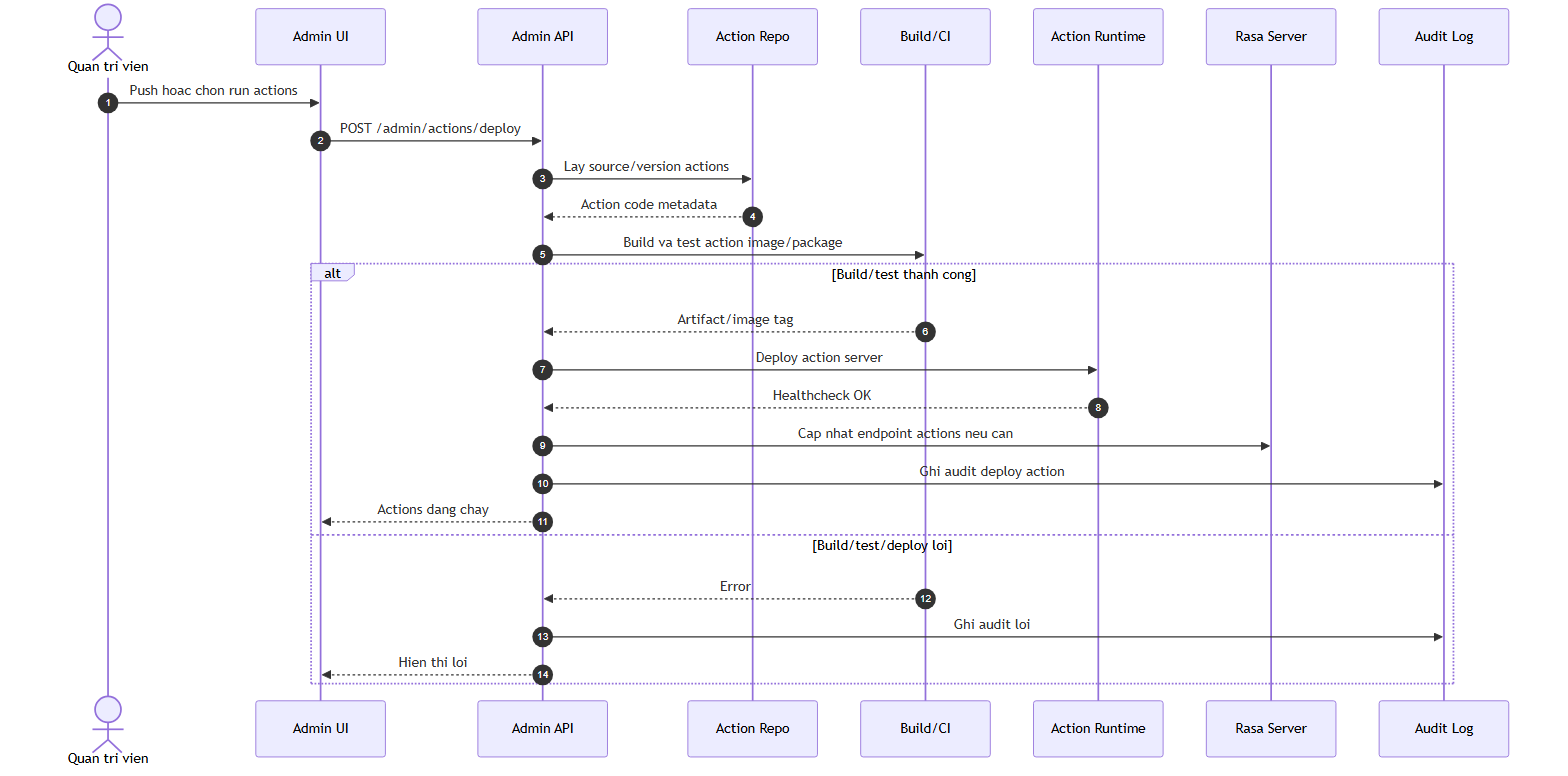
\includegraphics[width=\textwidth]{content/source/mermaid_sequence/seq_04.png}
    \caption{Luồng push/run actions}
\end{figure}

Về nghiệp vụ, quản trị viên cập nhật mã action hoặc lựa chọn action cần triển khai, hệ thống chuyển mã hoặc cấu hình mới tới backend, sau đó khởi động lại hoặc nạp lại action server để Rasa có thể gọi các action tương ứng. Sau khi action server chạy ổn định, chatbot mới có thể thực thi các bước nghiệp vụ cần truy cập dữ liệu bên ngoài hoặc tích hợp với KmaRAG.
